\subsection{PandaBoard (FM)}
\label{sec:panda}

\subsubsection{Overview}
\label{sec:panda-overview}
The modelcar hardware contains 4 PandaBoards intended for running the Engine Control Units (ECU) communicating with the SpeedDreams simulation, processing the simulation data and generating the servo commands.
While two PandaBoards are used by the simulation team to process the simulation data from SpeedDreams, another PandaBoard is used by our team to process the hardware control commands described in \autoref{sec:mqtt-car-control}.


\subsubsection{Requirements}
\label{sec:panda-req}
The following tasks were derived from the initial project description for the component running on the PandaBoard:
\begin{itemize}
    \item \textbf{TP1}: Install Genode with Fiasco.OC
    \item \textbf{TP2}: Develop MQTT client
    \item \textbf{TP3}: Convert control commands into concrete servo values
    \item \textbf{TP4}: Generate control commands
\end{itemize}

\paragraph{\textbf{TP1}} As operating system for the PandaBoard Genode running on top of the Fiasco.OS microkernel was used.
While there were less issues with running Genode on the PandaBoard compared to the Raspberry PI, a linux userland implementation of the PandaBoard component is also available in the \texttt{old/linux} folder and was used during initial development and testing.

\paragraph{\textbf{TP2}} As described in \autoref{sec:rpi-req} the same MQTT client based on the mosquitto library was used for the Raspberry Pi and the PandaBoard.
The PandaBoard subscribes to the \texttt{car-control} topic, processes received messages and then publishes to the \texttt{car-servo} topic.

\paragraph{\textbf{TP3}} The main purpose of the PandaBoard component is the transformation of generic control commands (eg. steer left, break) to concrete servo values. The format of the input and output messages is described in \autoref{sec:api} while the transformation is described in \autoref{sec:panda-genode}

\paragraph{\textbf{TP4}} To test the application independently of the SpeedDreams simulation, control commands can also be supplied directly as described in \autoref{sec:panda-testing}


\subsubsection{Genode application}
\label{sec:panda-genode}
The data from the SpeedDreams simulation is first received by the MQTT server on the \texttt{car-control} topic, as described in \autoref{sec:mqtt-car-control}.
The component running on the PandaBoard is subscribed to this MQTT topic and processes the information, see \autoref{sec:panda}.
The resulting commands are then published on the \texttt{car-servo} MQTT topic, described in \autoref{sec:mqtt-car-servo}.

% Two runfiles
% \autoref{fig:panda-genode}



\begin{figure}[h]
    \centering
    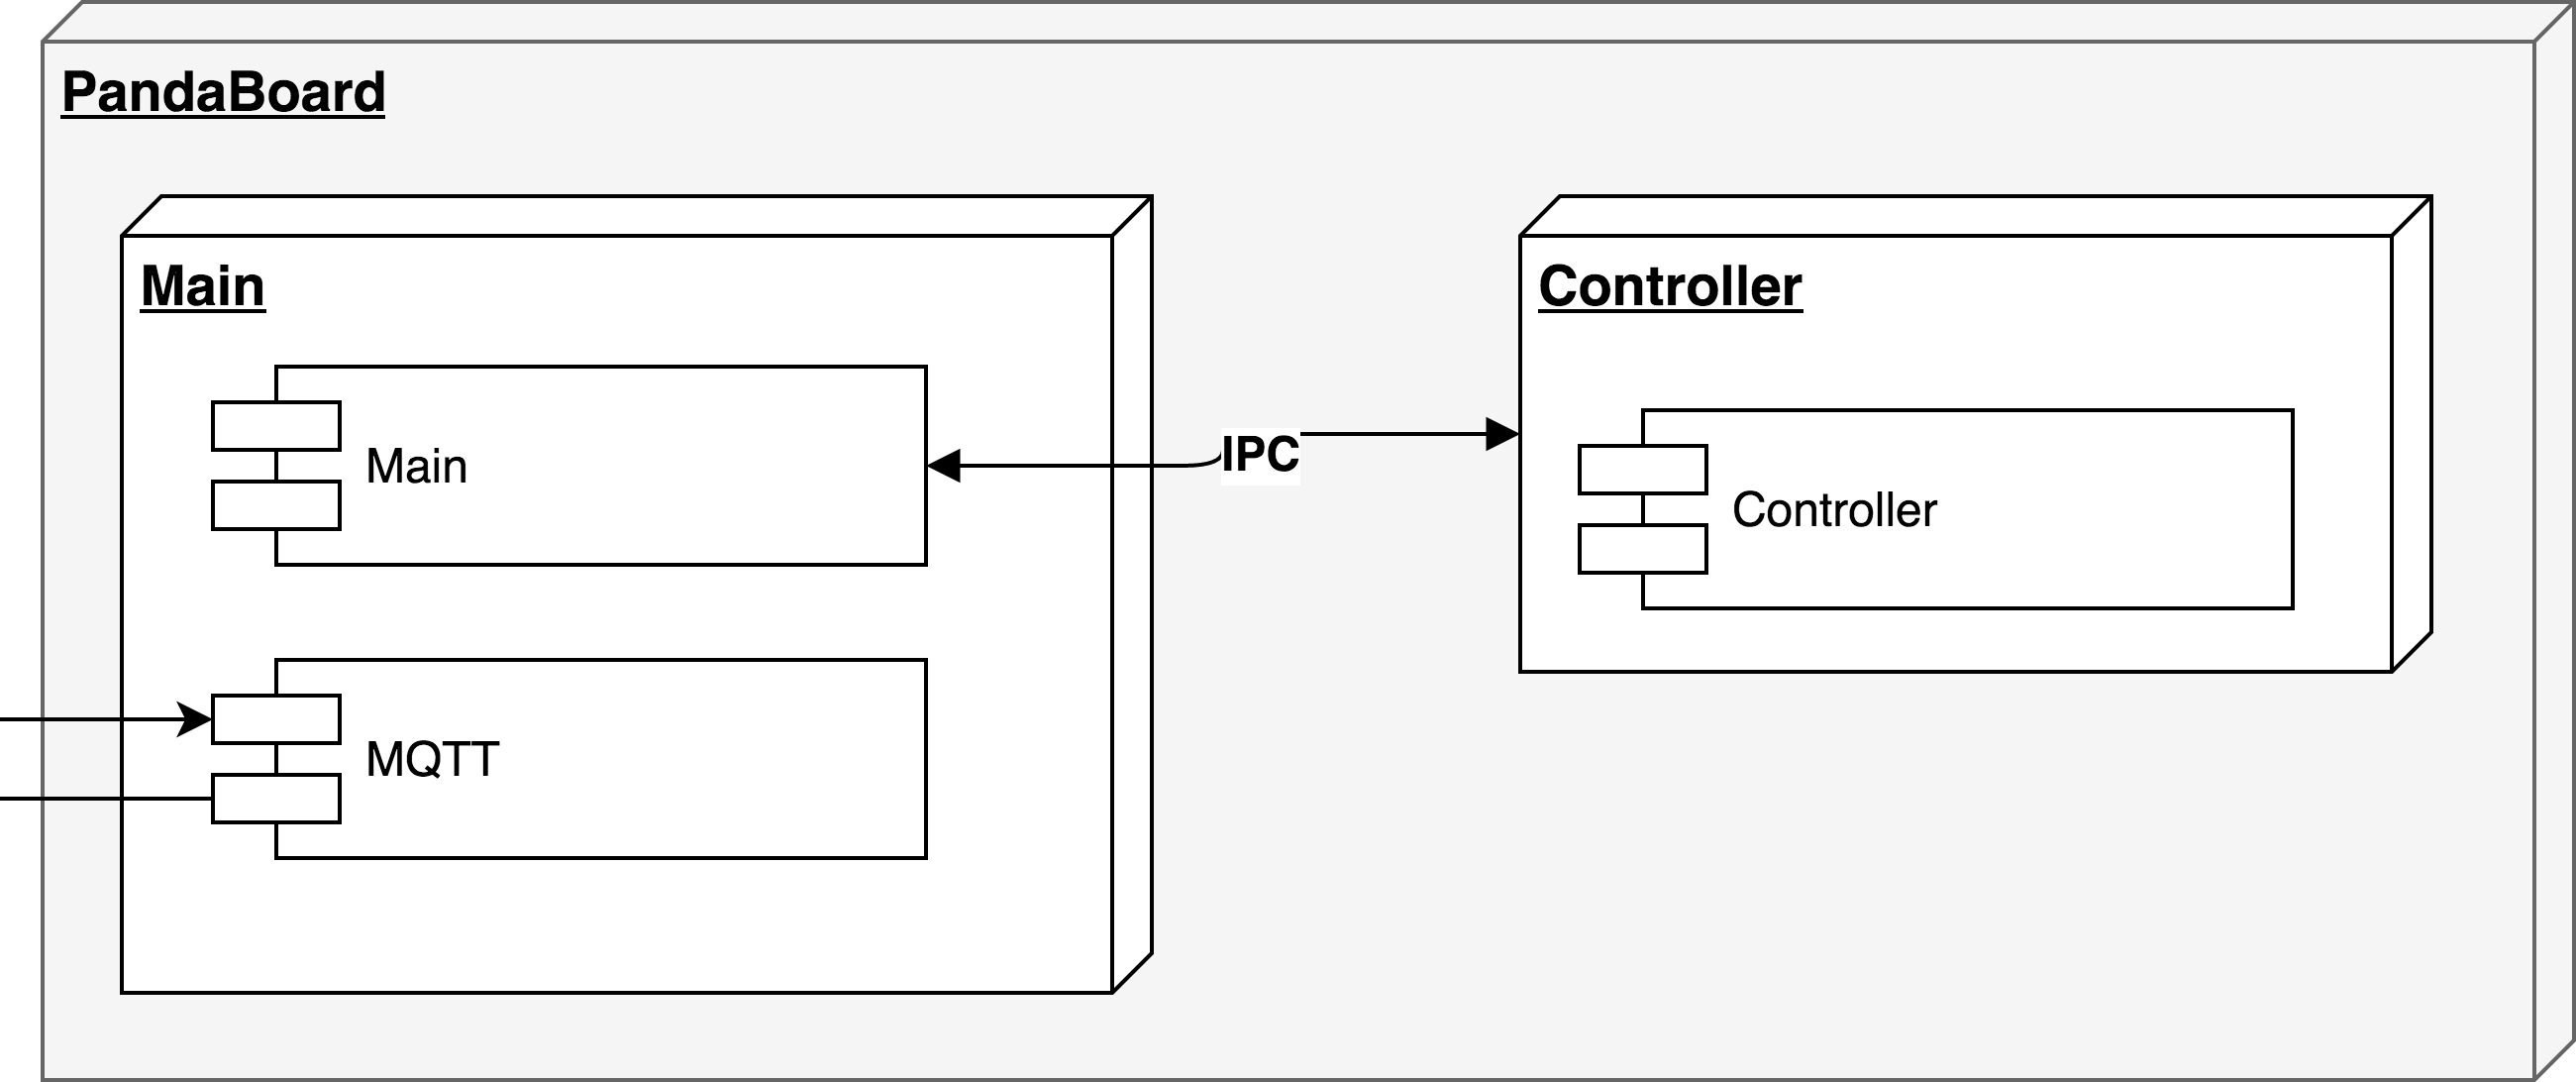
\includegraphics[width=0.7\linewidth]{images/comp_panda}
    \caption{Genode components of the PandaBoard}
    \label{fig:panda-genode}
\end{figure}

\subsubsection{Command processing}
\label{sec:panda-convert}

\subsubsection{Testing}
\label{sec:panda-testing}
To verify the data processing and the actuation of the hardware servos based on control commands sent to the \texttt{car-control} MQTT topic a test script was developed.
This way the hardware side of the hardware in the loop setup described in \autoref{sec:intro} can be tested independently of the software side developed by another project team.

The publish–subscribe pattern used by the MQTT server allows multiple clients to simultaneously connect to the server and subscribe to updates on a certain topic or publish messages to a certain topic.
In this style of communication there are no direct communication links and the components are loosely coupled, simplifying the testing of the interfaces between components.

By using the MQTT commandline tools available under Linux in the \texttt{mosquitto-clients} package message can easily be injected into the \texttt{car-control} topic without changing the configuration of any components.
\autoref{lst:panda-msgpub} shows a small test script that continiously sends steering control messages that cause the steering servos to alternate between actuation to the left and to the right. \\ % when processed by Panda, Rpi and servo components.

\begin{minipage}{\linewidth}
\begin{lstlisting}[style=mylistings, language=c, label=lst:panda-msgpub, caption=Injecting steering commands over MQTT]
#!/usr/bin/env bash
MQTT_IP=$1

while true; do
	mosquitto_pub -h $MQTT_IP -t 'car-control' -m '0,1.0'
	sleep 1
	mosquitto_pub -h $MQTT_IP -t 'car-control' -m '0,-1.0'
	sleep 1
done
\end{lstlisting}
\end{minipage} \\

In a similar manner the \texttt{mosquitto\_sub} commandline tool can be used to subscribe to MQTT topics. This provides easy access to the communication between components for debugging and testing purposes.
\autoref{lst:panda-msgsub} shows the command used to monitor the message published by the panda component. In both listings \texttt{\$MQTT\_IP} is a variable containing the IP address of the MQTT server. \\

\begin{minipage}{\linewidth}
\begin{lstlisting}[style=mylistings, language=c, label=lst:panda-msgsub, caption=Subscribing to MQTT topics]
mosquitto_sub -h $MQTT_IP -t 'car-servo'
\end{lstlisting}
\end{minipage} \\
